\par\Needspace{12\baselineskip}\SourceLeaf{288}%
\textls{Beweis}. Zuerst ist klar, dass der Winkel $(1)$ und die Linie $(2)(3)$ auf der innern Seite von $(1)(2)$ liegen; indem man also eine Linie durch $(1)$ sich so bewegen lässt, dass sie von $(1)(2)$ auf $(1)(3)$ übergeht, wird sie anfangs im Innern der Figur liegen. Gesetzt nun, dass sie in der Lage $(1)(3)$ nicht mehr ganz im Innern der Figur liege, so sei $(1)(u)$ diejenige Lage, bis wohin sie ganz im Innern liegt und dann aufhört, diese Eigenschaft zu haben; sie wird

\begin{center}\resizebox{6.0cm}{!}{%
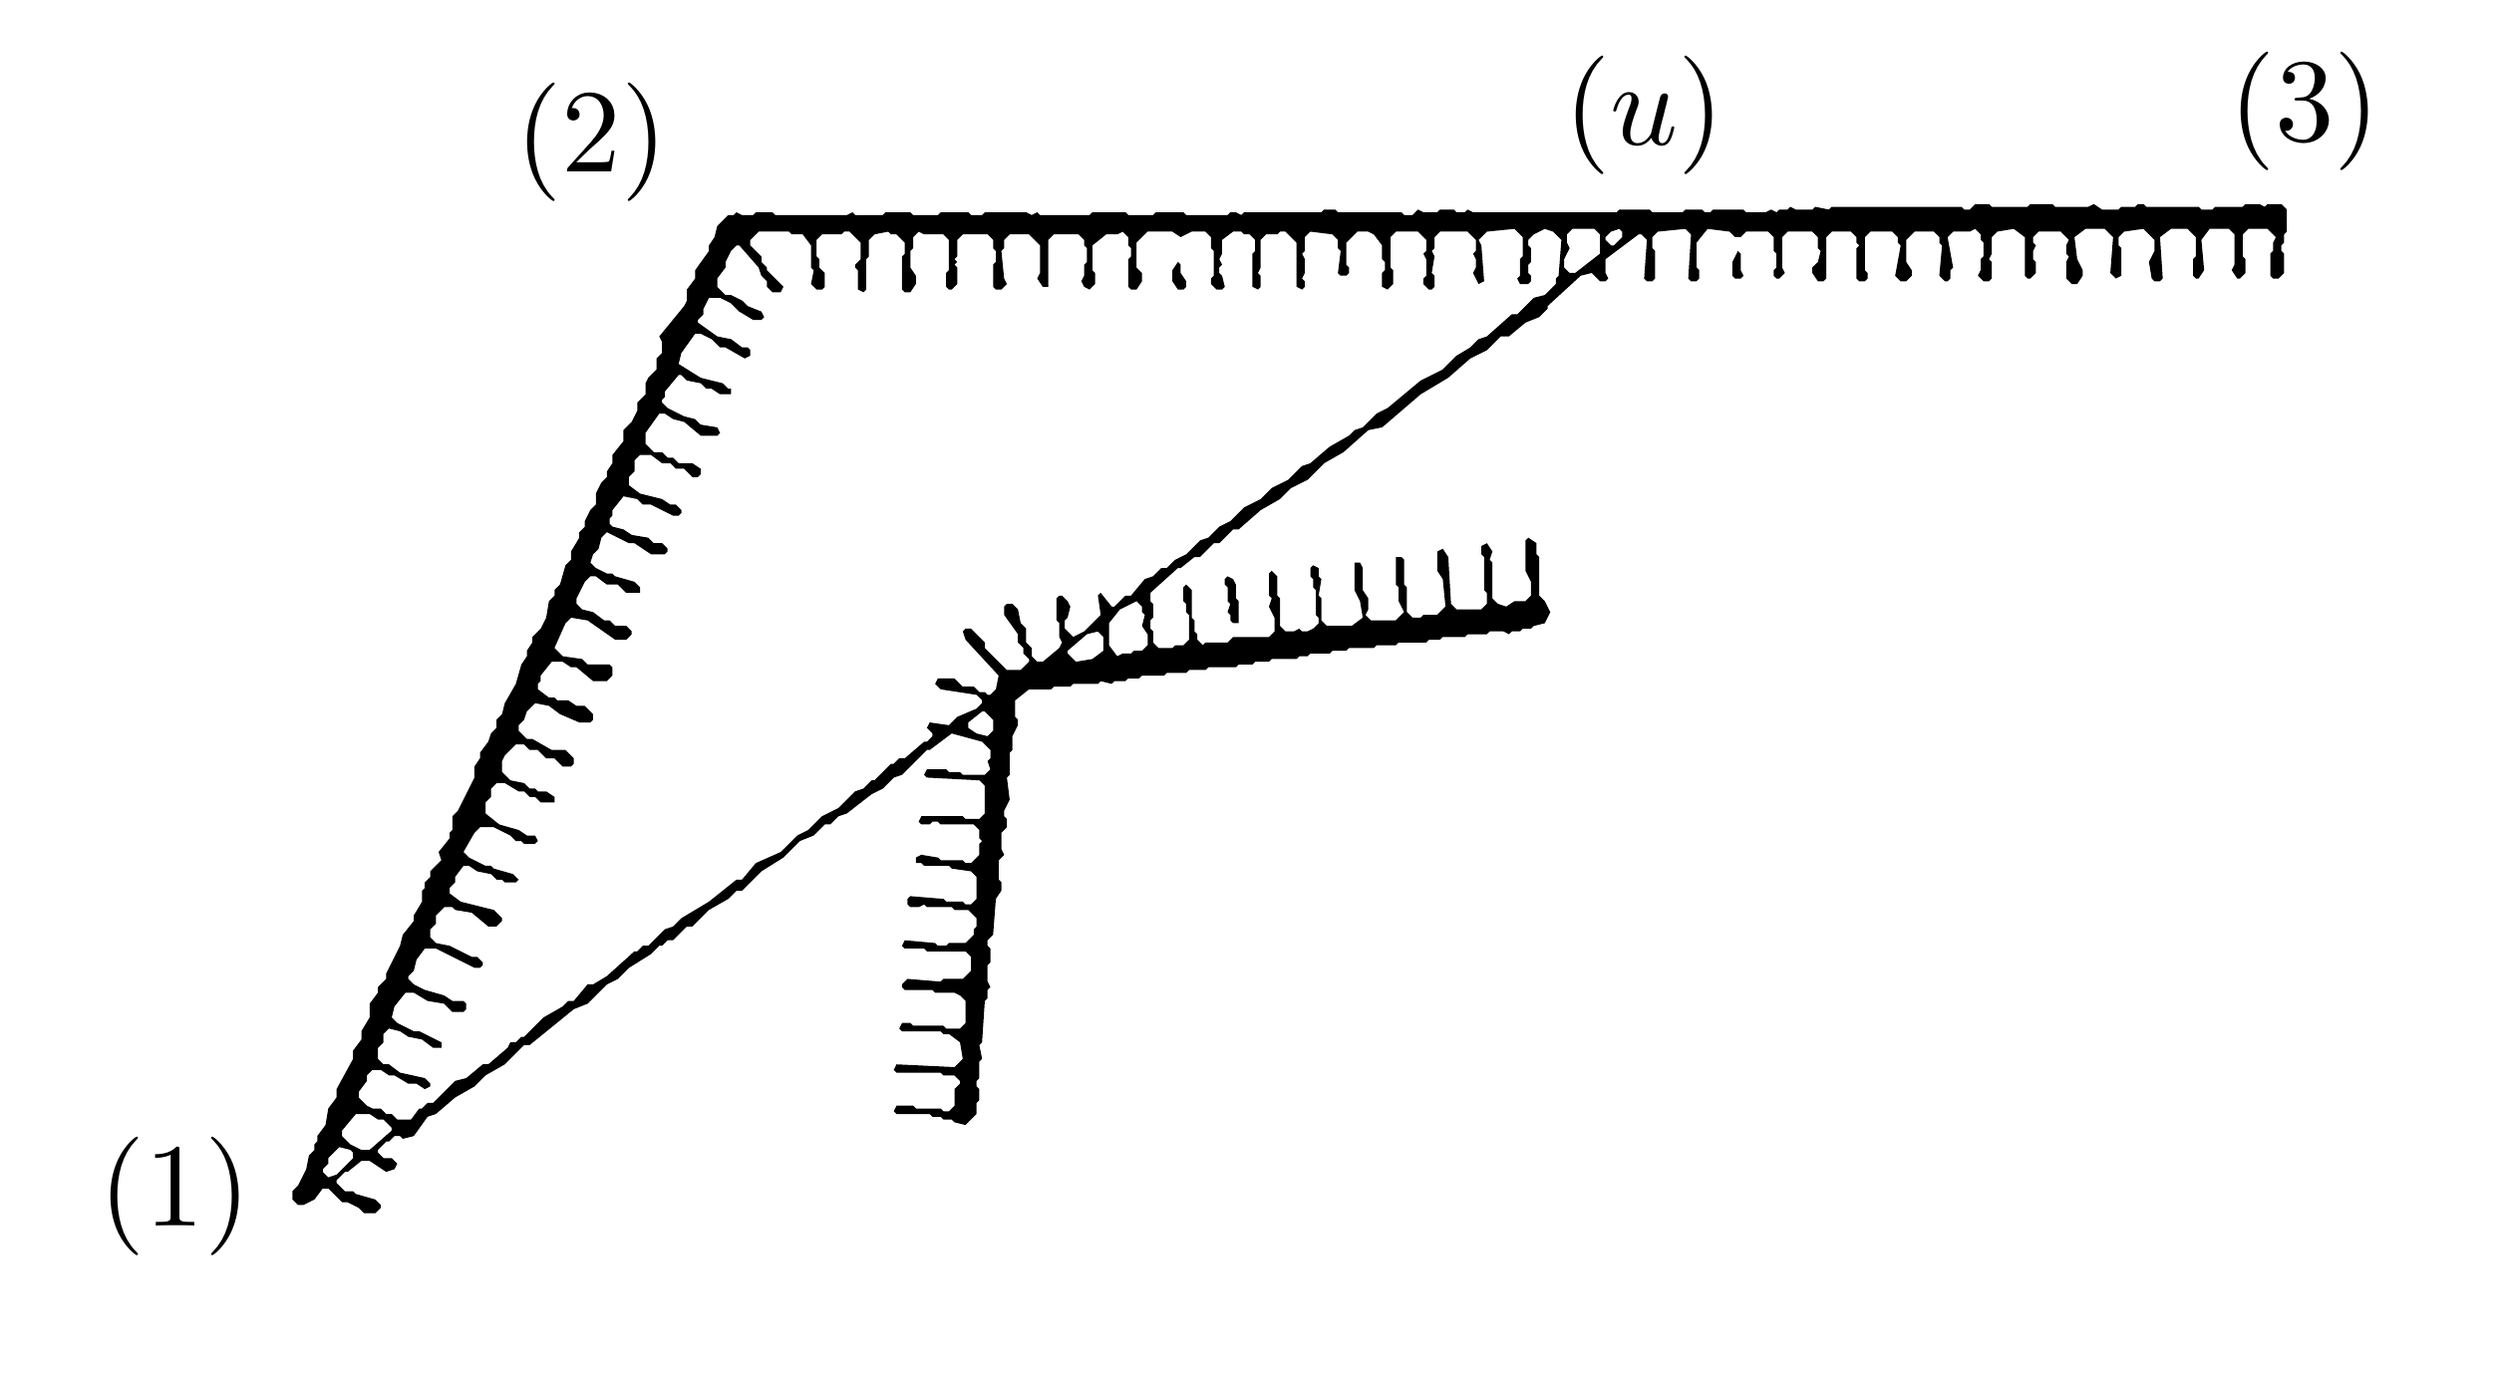
\begin{tikzpicture}[x=1pt,y=-1pt]
\path[use as bounding box] (0,0) rectangle (886,478);
\path[fill=black,draw=none,even odd rule]
(435,199) -- (434,200) -- (434,202) -- (435,203) -- (435,208) -- (436,209) -- (435,212) -- (436,213) -- (436,215) -- (437,216) -- (439,216) -- (439,208) -- (438,207) -- (438,202) -- (437,200) -- cycle
(620,81) -- (618,85) -- (618,90) -- (619,91) -- (621,91) -- (622,90) -- (621,88) -- (621,82) -- cycle
(819,66) -- (817,64) -- (812,64) -- (811,65) -- (809,64) -- (804,64) -- (803,65) -- (793,65) -- (792,66) -- (788,66) -- (787,65) -- (768,65) -- (767,64) -- (765,64) -- (764,65) -- (759,65) -- (758,66) -- (752,66) -- (749,64) -- (747,65) -- (735,65) -- (734,64) -- (726,64) -- (725,65) -- (712,65) -- (711,64) -- (706,64) -- (704,66) -- (702,66) -- (701,65) -- (654,65) -- (653,66) -- (648,65) -- (647,66) -- (641,66) -- (639,65) -- (638,66) -- (635,66) -- (634,67) -- (632,66) -- (630,67) -- (623,67) -- (622,66) -- (611,66) -- (610,67) -- (608,67) -- (607,66) -- (601,66) -- (600,67) -- (589,67) -- (588,66) -- (577,66) -- (576,67) -- (524,67) -- (522,66) -- (521,67) -- (518,67) -- (517,66) -- (512,66) -- (511,67) -- (506,67) -- (504,66) -- (502,68) -- (499,68) -- (498,67) -- (475,67) -- (474,66) -- (470,66) -- (469,67) -- (441,67) -- (440,68) -- (438,67) -- (436,67) -- (435,68) -- (420,68) -- (419,67) -- (409,67) -- (408,68) -- (399,68) -- (398,67) -- (386,67) -- (385,68) -- (367,68) -- (366,67) -- (364,68) -- (362,67) -- (347,67) -- (346,68) -- (342,68) -- (341,67) -- (331,67) -- (330,68) -- (321,68) -- (320,67) -- (311,67) -- (310,68) -- (300,68) -- (299,67) -- (297,68) -- (271,68) -- (270,67) -- (264,67) -- (263,68) -- (259,68) -- (257,67) -- (256,68) -- (254,68) -- (250,72) -- (249,76) -- (247,79) -- (247,81) -- (242,88) -- (242,91) -- (239,95) -- (239,99) -- (238,101) -- (229,112) -- (230,114) -- (230,118) -- (228,120) -- (228,124) -- (225,127) -- (224,129) -- (224,133) -- (221,136) -- (221,139) -- (219,143) -- (216,146) -- (216,150) -- (212,155) -- (212,158) -- (210,161) -- (210,163) -- (208,165) -- (206,169) -- (206,173) -- (204,175) -- (202,179) -- (202,181) -- (200,183) -- (200,185) -- (197,190) -- (197,193) -- (195,195) -- (193,202) -- (191,204) -- (191,206) -- (189,208) -- (188,214) -- (186,218) -- (183,221) -- (183,223) -- (181,226) -- (181,228) -- (179,231) -- (177,238) -- (173,245) -- (172,249) -- (170,251) -- (170,254) -- (168,256) -- (167,259) -- (164,263) -- (164,265) -- (162,268) -- (162,272) -- (156,284) -- (154,286) -- (154,291) -- (153,292) -- (153,294) -- (149,299) -- (150,302) -- (146,306) -- (146,308) -- (144,310) -- (144,312) -- (143,313) -- (143,317) -- (140,322) -- (140,324) -- (136,329) -- (135,333) -- (130,343) -- (130,345) -- (127,348) -- (127,350) -- (124,354) -- (124,359) -- (121,364) -- (121,367) -- (118,371) -- (118,374) -- (112,385) -- (112,388) -- (109,392) -- (108,398) -- (105,402) -- (105,404) -- (104,405) -- (104,407) -- (102,409) -- (101,414) -- (98,420) -- (96,422) -- (96,425) -- (98,427) -- (100,427) -- (104,425) -- (107,421) -- (109,421) -- (114,426) -- (116,426) -- (120,428) -- (122,430) -- (126,430) -- (128,428) -- (128,427) -- (126,425) -- (119,423) -- (118,422) -- (115,422) -- (112,419) -- (112,418) -- (115,415) -- (116,415) -- (121,411) -- (124,411) -- (130,415) -- (133,414) -- (134,412) -- (132,410) -- (129,410) -- (127,408) -- (127,407) -- (130,404) -- (131,404) -- (133,402) -- (135,402) -- (136,403) -- (140,402) -- (145,395) -- (148,394) -- (155,388) -- (162,384) -- (166,380) -- (173,376) -- (180,369) -- (182,369) -- (198,356) -- (203,354) -- (210,347) -- (214,345) -- (218,341) -- (226,336) -- (229,333) -- (230,333) -- (232,331) -- (234,331) -- (239,326) -- (241,326) -- (247,320) -- (254,316) -- (257,313) -- (259,313) -- (266,306) -- (274,301) -- (280,295) -- (285,293) -- (289,289) -- (291,289) -- (294,286) -- (297,285) -- (306,278) -- (310,276) -- (314,272) -- (317,271) -- (326,262) -- (327,262) -- (335,256) -- (346,259) -- (349,262) -- (349,265) -- (348,266) -- (349,269) -- (347,271) -- (339,271) -- (338,270) -- (334,270) -- (333,269) -- (326,269) -- (325,271) -- (326,272) -- (345,273) -- (347,275) -- (347,285) -- (345,287) -- (340,287) -- (339,286) -- (324,286) -- (323,288) -- (324,289) -- (327,289) -- (328,288) -- (330,288) -- (331,289) -- (343,289) -- (345,291) -- (345,294) -- (346,295) -- (345,296) -- (345,300) -- (342,303) -- (340,303) -- (339,302) -- (331,302) -- (330,301) -- (324,300) -- (322,301) -- (322,303) -- (324,303) -- (325,304) -- (334,304) -- (335,305) -- (342,306) -- (344,308) -- (344,316) -- (342,318) -- (340,318) -- (339,317) -- (333,317) -- (332,316) -- (320,315) -- (319,316) -- (319,318) -- (320,319) -- (323,319) -- (325,318) -- (326,319) -- (335,319) -- (336,320) -- (341,320) -- (344,323) -- (344,326) -- (343,327) -- (343,329) -- (340,332) -- (334,332) -- (333,333) -- (330,333) -- (329,332) -- (318,331) -- (317,333) -- (318,334) -- (325,334) -- (326,335) -- (340,335) -- (342,337) -- (342,342) -- (339,345) -- (332,345) -- (331,346) -- (319,345) -- (317,347) -- (317,348) -- (318,349) -- (328,349) -- (329,350) -- (336,350) -- (338,351) -- (340,353) -- (340,361) -- (338,363) -- (333,363) -- (332,362) -- (321,362) -- (320,361) -- (317,361) -- (316,363) -- (317,364) -- (331,364) -- (332,365) -- (334,365) -- (338,368) -- (339,374) -- (336,377) -- (315,376) -- (314,378) -- (315,379) -- (331,379) -- (332,380) -- (336,380) -- (338,382) -- (338,383) -- (336,385) -- (336,391) -- (334,393) -- (332,393) -- (331,392) -- (322,392) -- (321,391) -- (315,391) -- (314,393) -- (315,394) -- (327,394) -- (328,395) -- (331,395) -- (332,396) -- (335,396) -- (336,397) -- (340,398) -- (344,394) -- (344,390) -- (345,389) -- (345,385) -- (344,384) -- (344,382) -- (345,381) -- (345,375) -- (346,374) -- (345,369) -- (346,368) -- (347,353) -- (348,352) -- (348,349) -- (349,348) -- (348,346) -- (348,340) -- (349,339) -- (349,334) -- (348,333) -- (348,331) -- (350,329) -- (351,316) -- (353,313) -- (353,310) -- (352,309) -- (352,302) -- (354,300) -- (353,298) -- (353,292) -- (355,290) -- (355,287) -- (354,286) -- (354,284) -- (356,280) -- (355,272) -- (356,271) -- (356,263) -- (357,262) -- (357,257) -- (359,253) -- (359,251) -- (358,250) -- (358,244) -- (363,240) -- (371,240) -- (372,239) -- (378,239) -- (379,238) -- (388,238) -- (389,237) -- (393,238) -- (394,237) -- (398,237) -- (399,236) -- (403,236) -- (404,235) -- (412,235) -- (413,234) -- (420,234) -- (421,233) -- (427,233) -- (428,232) -- (438,232) -- (439,231) -- (444,231) -- (445,230) -- (450,230) -- (451,229) -- (460,229) -- (461,228) -- (464,228) -- (465,227) -- (472,227) -- (473,226) -- (478,226) -- (479,225) -- (488,225) -- (489,224) -- (496,224) -- (497,223) -- (507,223) -- (508,222) -- (512,222) -- (513,221) -- (521,221) -- (522,220) -- (529,220) -- (530,219) -- (535,219) -- (537,220) -- (538,219) -- (541,219) -- (542,218) -- (545,218) -- (546,217) -- (550,216) -- (552,212) -- (550,208) -- (548,206) -- (548,192) -- (547,191) -- (547,187) -- (544,185) -- (543,186) -- (543,197) -- (545,201) -- (545,206) -- (543,208) -- (539,208) -- (536,210) -- (533,209) -- (531,207) -- (531,194) -- (530,193) -- (531,190) -- (529,187) -- (527,188) -- (527,191) -- (528,192) -- (528,204) -- (529,205) -- (529,209) -- (527,211) -- (518,211) -- (516,209) -- (515,192) -- (513,189) -- (511,190) -- (511,197) -- (513,200) -- (514,210) -- (511,213) -- (506,213) -- (505,214) -- (502,214) -- (500,212) -- (500,203) -- (499,202) -- (499,193) -- (498,192) -- (496,192) -- (496,202) -- (497,203) -- (497,208) -- (499,212) -- (496,215) -- (487,215) -- (485,213) -- (486,211) -- (486,207) -- (484,204) -- (484,196) -- (483,194) -- (481,194) -- (481,204) -- (483,208) -- (484,214) -- (480,217) -- (471,217) -- (469,215) -- (469,207) -- (468,206) -- (469,200) -- (468,199) -- (468,196) -- (466,195) -- (465,196) -- (465,199) -- (466,200) -- (466,203) -- (467,204) -- (467,213) -- (468,214) -- (468,216) -- (466,218) -- (464,219) -- (462,219) -- (461,218) -- (459,219) -- (456,219) -- (454,217) -- (454,207) -- (453,206) -- (453,199) -- (451,197) -- (450,198) -- (450,206) -- (451,207) -- (450,210) -- (452,214) -- (452,219) -- (450,221) -- (437,221) -- (435,223) -- (427,223) -- (426,224) -- (424,222) -- (424,220) -- (423,219) -- (423,215) -- (422,214) -- (422,204) -- (420,202) -- (419,203) -- (419,208) -- (420,209) -- (420,212) -- (421,213) -- (421,222) -- (419,224) -- (416,224) -- (415,225) -- (410,225) -- (408,223) -- (408,219) -- (407,218) -- (407,215) -- (408,214) -- (408,209) -- (407,208) -- (407,205) -- (417,196) -- (418,196) -- (423,192) -- (425,192) -- (430,187) -- (432,187) -- (437,182) -- (439,182) -- (447,175) -- (454,171) -- (458,167) -- (464,164) -- (470,158) -- (477,154) -- (486,146) -- (491,145) -- (505,133) -- (515,127) -- (523,120) -- (529,117) -- (534,112) -- (537,112) -- (543,107) -- (548,105) -- (551,102) -- (551,101) -- (563,90) -- (567,89) -- (570,92) -- (572,92) -- (573,91) -- (572,89) -- (572,84) -- (584,75) -- (585,75) -- (587,77) -- (586,91) -- (587,92) -- (589,92) -- (590,91) -- (590,81) -- (589,80) -- (589,76) -- (591,74) -- (601,73) -- (603,75) -- (602,91) -- (603,92) -- (605,92) -- (606,91) -- (606,88) -- (605,87) -- (605,78) -- (609,73) -- (617,74) -- (619,76) -- (621,76) -- (623,74) -- (631,74) -- (633,76) -- (633,81) -- (634,82) -- (634,87) -- (633,88) -- (633,90) -- (634,91) -- (635,91) -- (637,89) -- (636,87) -- (636,76) -- (638,74) -- (647,74) -- (649,76) -- (649,80) -- (650,81) -- (649,85) -- (647,87) -- (647,89) -- (649,92) -- (651,92) -- (652,91) -- (652,76) -- (654,74) -- (661,74) -- (663,76) -- (663,78) -- (664,79) -- (663,80) -- (663,91) -- (664,92) -- (666,92) -- (667,91) -- (667,89) -- (666,88) -- (666,76) -- (668,74) -- (676,74) -- (678,76) -- (678,78) -- (679,79) -- (677,90) -- (679,92) -- (681,92) -- (683,90) -- (683,88) -- (681,85) -- (681,77) -- (684,74) -- (691,74) -- (693,76) -- (693,78) -- (694,79) -- (693,90) -- (695,92) -- (696,92) -- (697,91) -- (697,88) -- (698,87) -- (696,76) -- (698,74) -- (704,74) -- (706,73) -- (708,75) -- (708,77) -- (709,78) -- (709,83) -- (708,84) -- (708,88) -- (707,90) -- (709,92) -- (711,92) -- (712,91) -- (712,85) -- (711,84) -- (712,82) -- (712,76) -- (714,74) -- (720,73) -- (724,76) -- (724,90) -- (725,91) -- (726,91) -- (728,89) -- (728,85) -- (727,84) -- (727,81) -- (728,79) -- (727,78) -- (727,76) -- (729,74) -- (737,74) -- (740,77) -- (739,79) -- (739,82) -- (740,83) -- (739,85) -- (739,91) -- (741,93) -- (743,93) -- (745,90) -- (745,88) -- (743,84) -- (742,76) -- (746,73) -- (753,73) -- (756,76) -- (755,89) -- (757,91) -- (759,90) -- (759,80) -- (758,79) -- (758,76) -- (760,74) -- (767,73) -- (771,77) -- (771,81) -- (769,85) -- (770,91) -- (771,92) -- (773,92) -- (774,91) -- (773,76) -- (777,73) -- (783,73) -- (786,76) -- (786,83) -- (785,84) -- (785,90) -- (786,91) -- (787,91) -- (789,88) -- (788,77) -- (791,73) -- (798,73) -- (800,75) -- (800,86) -- (799,88) -- (801,91) -- (802,91) -- (804,89) -- (804,84) -- (803,83) -- (803,75) -- (805,73) -- (812,73) -- (815,76) -- (814,78) -- (814,81) -- (813,82) -- (813,90) -- (814,91) -- (816,91) -- (818,89) -- (818,82) -- (817,81) -- (817,79) -- (818,78) -- (818,75) -- (819,74) -- cycle
(117,407) -- (118,408) -- (118,410) -- (112,416) -- (109,417) -- (107,415) -- (107,414) -- (109,412) -- (109,410) -- (113,406) -- cycle
(114,402) -- (114,400) -- (119,394) -- (124,394) -- (127,396) -- (129,396) -- (132,399) -- (132,400) -- (124,407) -- (121,407) -- (117,405) -- cycle
(346,248) -- (347,248) -- (350,251) -- (350,255) -- (348,257) -- (344,256) -- (341,254) -- (341,252) -- cycle
(388,219) -- (390,221) -- (390,226) -- (386,229) -- (380,230) -- (377,227) -- (377,226) -- (384,220) -- cycle
(402,208) -- (404,210) -- (404,212) -- (405,213) -- (404,217) -- (406,220) -- (406,224) -- (404,226) -- (401,226) -- (400,227) -- (397,227) -- (395,228) -- (392,224) -- (392,216) -- (396,211) -- cycle
(577,73) -- (578,74) -- (578,76) -- (575,79) -- (574,79) -- (572,77) -- (572,76) -- (574,74) -- cycle
(568,73) -- (570,75) -- (570,82) -- (561,89) -- (559,89) -- (557,87) -- (557,84) -- (559,80) -- (558,78) -- (558,75) -- (560,73) -- cycle
(556,77) -- (555,90) -- (554,91) -- (554,93) -- (550,97) -- (546,98) -- (540,104) -- (538,104) -- (529,112) -- (526,113) -- (523,116) -- (518,119) -- (513,124) -- (505,128) -- (493,138) -- (489,140) -- (484,145) -- (481,146) -- (479,148) -- (472,152) -- (465,158) -- (462,159) -- (457,164) -- (451,167) -- (447,171) -- (441,174) -- (436,179) -- (432,181) -- (428,185) -- (425,186) -- (420,191) -- (416,193) -- (413,196) -- (411,196) -- (408,199) -- (405,200) -- (400,206) -- (398,206) -- (394,210) -- (393,210) -- (389,205) -- (388,206) -- (389,213) -- (383,219) -- (379,221) -- (376,218) -- (376,215) -- (377,214) -- (378,210) -- (377,208) -- (375,206) -- (374,206) -- (373,207) -- (373,215) -- (374,216) -- (374,221) -- (375,223) -- (374,225) -- (368,230) -- (366,230) -- (364,228) -- (364,225) -- (362,223) -- (362,218) -- (360,216) -- (359,211) -- (357,209) -- (355,209) -- (354,210) -- (354,213) -- (359,220) -- (359,223) -- (361,225) -- (361,227) -- (363,229) -- (363,230) -- (360,233) -- (355,233) -- (347,225) -- (347,223) -- (342,218) -- (340,218) -- (339,219) -- (340,222) -- (352,235) -- (351,240) -- (349,242) -- (348,242) -- (347,241) -- (345,241) -- (343,239) -- (339,239) -- (336,236) -- (330,236) -- (329,238) -- (331,240) -- (344,242) -- (346,244) -- (346,245) -- (344,247) -- (337,250) -- (334,253) -- (327,252) -- (326,254) -- (328,256) -- (328,257) -- (326,259) -- (325,259) -- (318,265) -- (316,265) -- (314,267) -- (313,267) -- (307,273) -- (306,273) -- (303,276) -- (300,277) -- (294,283) -- (288,286) -- (283,291) -- (279,293) -- (273,299) -- (264,303) -- (259,309) -- (257,309) -- (247,317) -- (237,323) -- (234,326) -- (231,327) -- (225,333) -- (223,333) -- (221,335) -- (220,335) -- (210,344) -- (205,347) -- (203,347) -- (198,353) -- (196,353) -- (194,355) -- (187,359) -- (180,366) -- (179,366) -- (177,368) -- (175,368) -- (174,370) -- (167,376) -- (165,376) -- (159,381) -- (155,382) -- (147,390) -- (145,390) -- (143,392) -- (142,392) -- (139,396) -- (134,396) -- (132,394) -- (130,394) -- (128,392) -- (125,392) -- (123,391) -- (120,388) -- (120,386) -- (123,382) -- (123,380) -- (125,378) -- (128,378) -- (131,380) -- (133,380) -- (138,383) -- (141,383) -- (144,385) -- (146,384) -- (146,383) -- (144,381) -- (135,379) -- (131,376) -- (129,376) -- (127,374) -- (127,370) -- (129,368) -- (129,365) -- (131,363) -- (135,364) -- (138,366) -- (143,367) -- (147,370) -- (150,370) -- (150,368) -- (142,364) -- (140,364) -- (134,361) -- (132,359) -- (133,355) -- (137,350) -- (140,350) -- (145,353) -- (151,354) -- (154,357) -- (158,357) -- (159,356) -- (159,354) -- (158,353) -- (154,353) -- (151,351) -- (144,349) -- (140,347) -- (138,345) -- (138,344) -- (140,342) -- (141,338) -- (144,334) -- (148,334) -- (162,341) -- (164,341) -- (165,340) -- (165,339) -- (163,337) -- (161,337) -- (153,333) -- (148,332) -- (146,330) -- (146,327) -- (148,325) -- (148,322) -- (151,319) -- (154,319) -- (155,320) -- (161,321) -- (167,326) -- (170,326) -- (172,324) -- (172,323) -- (169,320) -- (157,317) -- (153,314) -- (153,312) -- (155,310) -- (155,308) -- (158,304) -- (160,304) -- (163,306) -- (168,307) -- (170,309) -- (172,309) -- (173,310) -- (177,310) -- (178,309) -- (176,307) -- (169,305) -- (168,304) -- (166,304) -- (160,301) -- (158,299) -- (162,292) -- (164,290) -- (169,290) -- (175,293) -- (177,295) -- (179,295) -- (180,296) -- (184,296) -- (185,295) -- (184,293) -- (181,293) -- (178,291) -- (171,289) -- (166,285) -- (166,281) -- (168,279) -- (168,276) -- (170,274) -- (173,274) -- (178,277) -- (180,277) -- (182,279) -- (184,279) -- (186,281) -- (191,281) -- (191,279) -- (188,277) -- (185,277) -- (184,276) -- (182,276) -- (180,274) -- (175,273) -- (172,270) -- (172,266) -- (173,264) -- (177,260) -- (180,260) -- (182,262) -- (185,262) -- (188,265) -- (191,265) -- (194,268) -- (197,268) -- (198,267) -- (198,265) -- (195,262) -- (190,262) -- (183,258) -- (181,258) -- (178,255) -- (178,253) -- (180,251) -- (181,248) -- (184,245) -- (189,246) -- (193,249) -- (200,252) -- (204,252) -- (205,251) -- (205,249) -- (202,246) -- (199,246) -- (196,244) -- (192,244) -- (191,243) -- (189,243) -- (185,240) -- (185,238) -- (186,237) -- (186,235) -- (190,230) -- (194,230) -- (197,232) -- (199,232) -- (205,237) -- (210,237) -- (212,235) -- (212,232) -- (211,231) -- (203,231) -- (201,229) -- (194,228) -- (191,225) -- (195,216) -- (197,214) -- (203,215) -- (213,222) -- (217,222) -- (219,220) -- (219,219) -- (217,217) -- (213,217) -- (211,215) -- (209,215) -- (205,212) -- (201,211) -- (199,209) -- (199,207) -- (202,201) -- (204,199) -- (206,199) -- (210,202) -- (214,202) -- (217,205) -- (222,205) -- (222,203) -- (220,201) -- (213,199) -- (212,198) -- (210,198) -- (206,196) -- (204,194) -- (205,191) -- (207,189) -- (208,185) -- (210,183) -- (218,187) -- (220,187) -- (226,191) -- (231,191) -- (232,190) -- (232,189) -- (230,187) -- (227,187) -- (225,185) -- (219,184) -- (216,182) -- (212,181) -- (211,180) -- (211,178) -- (212,177) -- (212,175) -- (216,170) -- (221,171) -- (223,173) -- (226,173) -- (234,177) -- (236,177) -- (237,176) -- (237,175) -- (235,173) -- (233,173) -- (230,171) -- (222,169) -- (218,166) -- (218,163) -- (220,161) -- (220,157) -- (222,155) -- (226,155) -- (230,158) -- (233,158) -- (235,160) -- (238,160) -- (241,163) -- (243,163) -- (244,162) -- (244,160) -- (241,158) -- (236,158) -- (234,156) -- (232,156) -- (230,154) -- (227,154) -- (224,151) -- (224,147) -- (229,140) -- (231,140) -- (234,142) -- (238,143) -- (244,148) -- (250,148) -- (251,147) -- (250,145) -- (244,144) -- (242,142) -- (238,141) -- (232,138) -- (230,136) -- (230,135) -- (231,134) -- (231,132) -- (236,126) -- (237,126) -- (239,128) -- (244,129) -- (246,131) -- (248,131) -- (251,133) -- (255,133) -- (255,131) -- (254,131) -- (252,129) -- (244,127) -- (236,122) -- (237,118) -- (242,111) -- (244,111) -- (248,113) -- (251,116) -- (253,116) -- (260,120) -- (262,119) -- (262,117) -- (261,116) -- (259,116) -- (255,113) -- (250,112) -- (243,107) -- (243,106) -- (245,104) -- (245,102) -- (247,98) -- (251,98) -- (255,100) -- (258,103) -- (263,106) -- (266,106) -- (267,105) -- (266,103) -- (261,101) -- (259,99) -- (255,97) -- (253,97) -- (250,94) -- (250,91) -- (253,87) -- (253,85) -- (255,81) -- (257,79) -- (258,79) -- (265,87) -- (266,90) -- (268,92) -- (268,94) -- (270,96) -- (273,96) -- (274,94) -- (268,88) -- (268,87) -- (266,85) -- (266,83) -- (262,79) -- (262,77) -- (265,74) -- (276,74) -- (277,75) -- (281,75) -- (284,79) -- (284,87) -- (285,88) -- (284,93) -- (286,95) -- (288,95) -- (289,94) -- (289,89) -- (287,87) -- (287,84) -- (286,83) -- (286,77) -- (288,75) -- (295,75) -- (296,74) -- (298,74) -- (302,78) -- (302,84) -- (300,86) -- (300,87) -- (301,88) -- (301,95) -- (303,96) -- (304,95) -- (304,84) -- (305,83) -- (305,77) -- (307,75) -- (312,74) -- (313,75) -- (315,75) -- (318,78) -- (318,82) -- (317,83) -- (317,95) -- (318,96) -- (320,96) -- (322,93) -- (322,90) -- (320,87) -- (320,81) -- (321,80) -- (321,76) -- (323,74) -- (325,75) -- (332,75) -- (334,77) -- (334,88) -- (333,89) -- (333,94) -- (334,95) -- (335,95) -- (337,93) -- (337,87) -- (336,86) -- (337,85) -- (336,84) -- (337,83) -- (337,77) -- (339,75) -- (348,75) -- (350,77) -- (350,80) -- (351,81) -- (351,85) -- (350,86) -- (350,94) -- (351,95) -- (353,95) -- (355,93) -- (354,91) -- (353,81) -- (354,80) -- (354,77) -- (356,75) -- (363,75) -- (367,79) -- (367,89) -- (366,91) -- (368,94) -- (370,94) -- (370,77) -- (372,75) -- (381,75) -- (383,77) -- (383,79) -- (384,80) -- (384,85) -- (383,86) -- (383,90) -- (382,92) -- (383,94) -- (385,95) -- (387,93) -- (387,89) -- (386,88) -- (386,79) -- (391,75) -- (395,75) -- (397,74) -- (399,76) -- (399,79) -- (400,80) -- (400,83) -- (399,84) -- (399,94) -- (400,95) -- (402,95) -- (404,92) -- (404,89) -- (402,87) -- (402,78) -- (406,74) -- (415,74) -- (418,76) -- (422,74) -- (427,74) -- (429,76) -- (429,80) -- (430,81) -- (430,90) -- (429,91) -- (429,93) -- (431,95) -- (433,95) -- (434,94) -- (433,90) -- (432,89) -- (432,87) -- (433,86) -- (432,84) -- (433,82) -- (433,77) -- (437,74) -- (440,74) -- (441,75) -- (443,75) -- (445,77) -- (445,81) -- (444,82) -- (444,94) -- (446,95) -- (447,94) -- (447,90) -- (446,89) -- (447,87) -- (447,77) -- (449,75) -- (453,75) -- (454,74) -- (456,74) -- (460,78) -- (460,94) -- (462,95) -- (463,94) -- (463,92) -- (462,91) -- (463,89) -- (463,84) -- (462,82) -- (463,81) -- (463,76) -- (465,74) -- (473,75) -- (475,77) -- (475,80) -- (476,81) -- (475,89) -- (476,90) -- (478,90) -- (479,89) -- (479,87) -- (478,86) -- (478,78) -- (482,74) -- (486,74) -- (488,75) -- (491,79) -- (491,84) -- (492,85) -- (492,88) -- (491,89) -- (491,94) -- (493,95) -- (495,93) -- (495,88) -- (494,87) -- (494,76) -- (496,74) -- (504,74) -- (507,77) -- (507,81) -- (506,82) -- (507,84) -- (507,90) -- (506,91) -- (506,93) -- (508,95) -- (509,95) -- (510,94) -- (510,90) -- (509,89) -- (510,83) -- (509,81) -- (510,80) -- (510,76) -- (512,74) -- (522,74) -- (525,77) -- (525,81) -- (524,82) -- (525,84) -- (525,87) -- (524,89) -- (526,93) -- (528,92) -- (527,79) -- (526,77) -- (529,74) -- (539,73) -- (542,76) -- (542,83) -- (541,84) -- (541,90) -- (540,91) -- (541,93) -- (544,93) -- (545,92) -- (545,90) -- (544,89) -- (544,86) -- (545,85) -- (545,80) -- (544,79) -- (544,77) -- (546,75) -- (550,73) -- (553,74) -- cycle
(417,85) -- (415,88) -- (415,92) -- (417,95) -- (419,95) -- (420,94) -- (420,92) -- (418,89) -- (418,86) -- cycle;
\node[inner sep=0pt,font=\fontsize{10}{12}\selectfont] at (53.50,424.00) {\scalebox{4.3}{$(1)$}};
\node[inner sep=0pt,font=\fontsize{10}{12}\selectfont] at (204.50,41.50) {\scalebox{4.3}{$(2)$}};
\node[inner sep=0pt,font=\fontsize{10}{12}\selectfont] at (586.00,32.00) {\scalebox{4.3}{$(u)$}};
\node[inner sep=0pt,font=\fontsize{10}{12}\selectfont] at (825.50,30.50) {\scalebox{4.3}{$(3)$}};
\end{tikzpicture}%
}
\hfill\resizebox{6.5cm}{!}{%
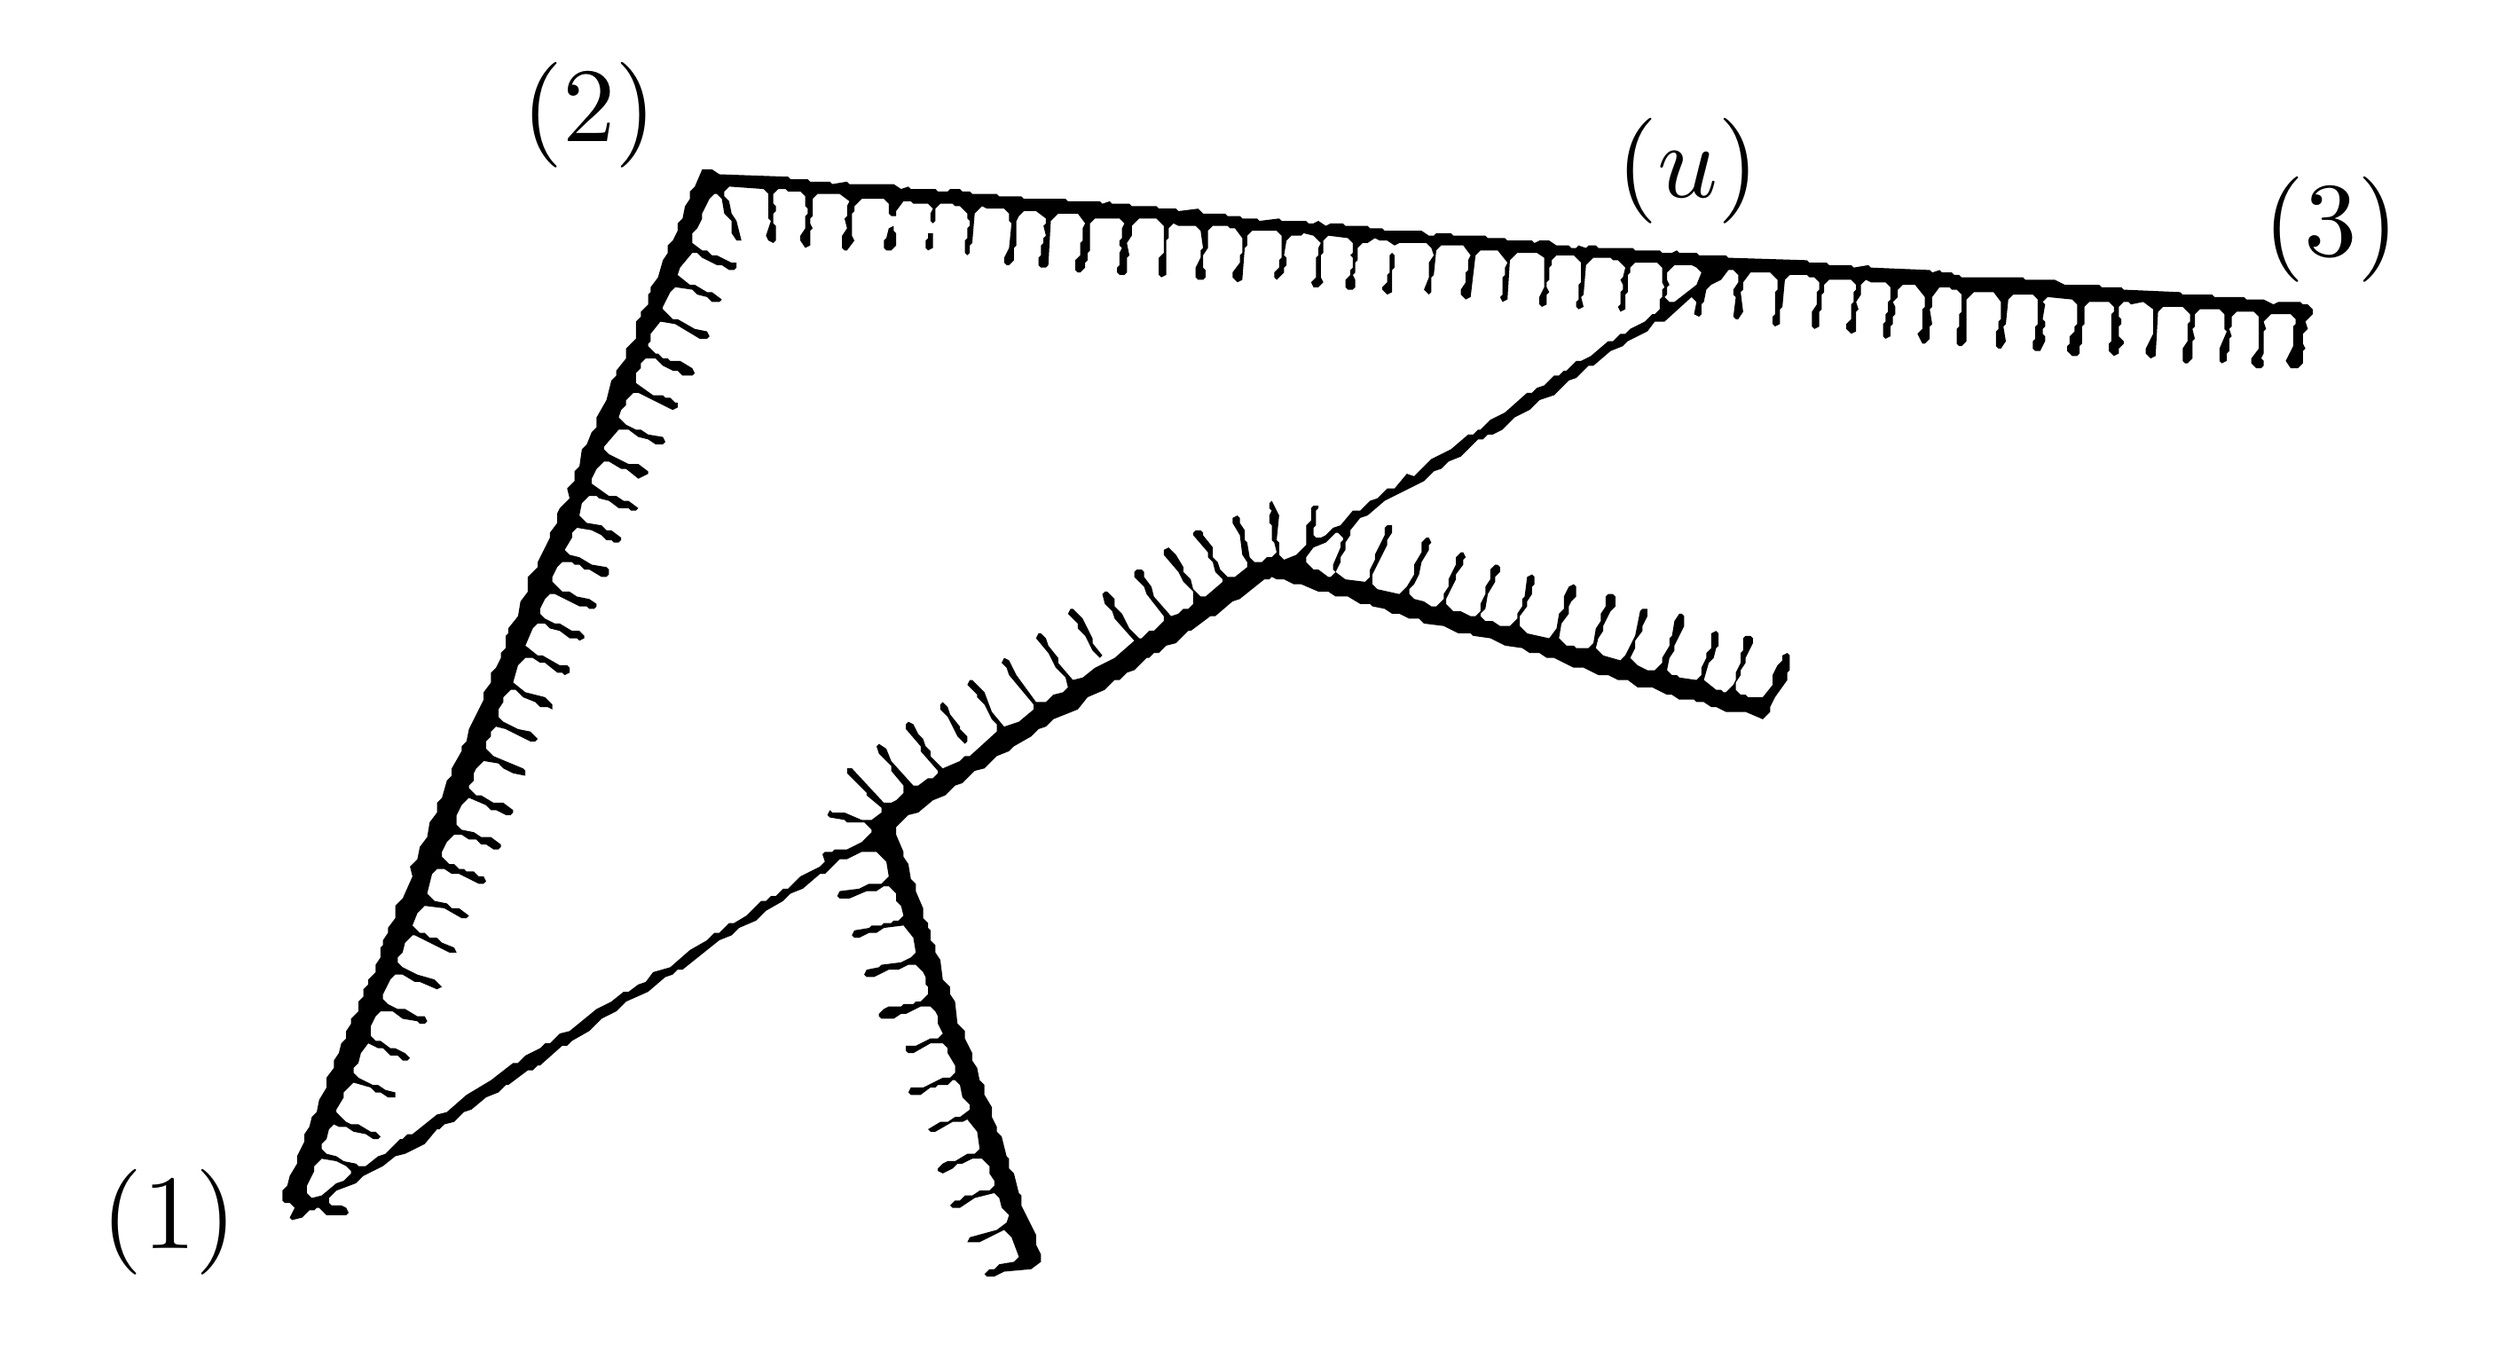
\begin{tikzpicture}[x=1pt,y=-1pt]
\path[use as bounding box] (0,0) rectangle (998,530);
\path[fill=black,draw=none,even odd rule]
(108,486) -- (109,487) -- (113,486) -- (116,483) -- (118,483) -- (119,482) -- (120,482) -- (123,485) -- (131,485) -- (132,484) -- (131,482) -- (129,481) -- (125,481) -- (124,480) -- (124,478) -- (127,475) -- (135,472) -- (138,469) -- (146,465) -- (151,461) -- (155,460) -- (163,456) -- (168,450) -- (169,450) -- (171,448) -- (175,447) -- (179,443) -- (182,442) -- (188,437) -- (193,435) -- (196,432) -- (197,432) -- (205,426) -- (207,426) -- (209,424) -- (210,424) -- (219,416) -- (221,416) -- (223,414) -- (230,410) -- (235,405) -- (241,402) -- (245,398) -- (254,394) -- (261,388) -- (264,387) -- (266,385) -- (268,385) -- (283,373) -- (288,371) -- (291,368) -- (298,365) -- (302,361) -- (309,357) -- (312,354) -- (317,352) -- (324,346) -- (326,346) -- (332,340) -- (335,340) -- (341,337) -- (347,337) -- (351,341) -- (352,347) -- (349,350) -- (344,350) -- (340,352) -- (332,353) -- (331,355) -- (332,356) -- (336,356) -- (343,353) -- (347,353) -- (350,351) -- (352,351) -- (355,354) -- (355,357) -- (357,359) -- (358,363) -- (356,365) -- (354,365) -- (353,366) -- (350,366) -- (349,367) -- (345,367) -- (344,368) -- (338,369) -- (337,371) -- (338,372) -- (340,372) -- (344,370) -- (347,370) -- (350,368) -- (358,367) -- (362,372) -- (363,378) -- (361,380) -- (357,382) -- (349,383) -- (348,384) -- (343,385) -- (342,387) -- (343,388) -- (346,388) -- (352,385) -- (356,385) -- (360,383) -- (363,383) -- (366,386) -- (367,388) -- (367,391) -- (368,392) -- (368,395) -- (365,398) -- (363,398) -- (362,399) -- (358,399) -- (357,400) -- (352,400) -- (350,401) -- (348,403) -- (348,404) -- (349,405) -- (354,405) -- (357,403) -- (359,403) -- (365,400) -- (369,400) -- (371,402) -- (372,404) -- (372,407) -- (374,411) -- (372,413) -- (369,413) -- (363,416) -- (359,416) -- (359,418) -- (360,419) -- (362,419) -- (369,415) -- (374,415) -- (376,417) -- (376,419) -- (379,424) -- (379,427) -- (377,429) -- (374,429) -- (366,433) -- (361,433) -- (360,435) -- (361,436) -- (365,436) -- (369,433) -- (371,433) -- (372,432) -- (376,432) -- (378,430) -- (379,430) -- (381,432) -- (382,437) -- (385,440) -- (385,442) -- (381,445) -- (379,445) -- (376,447) -- (373,447) -- (368,450) -- (369,451) -- (371,451) -- (378,447) -- (382,447) -- (384,446) -- (388,451) -- (389,458) -- (387,460) -- (384,460) -- (379,463) -- (376,463) -- (374,464) -- (372,466) -- (372,467) -- (374,468) -- (378,466) -- (380,464) -- (382,464) -- (386,462) -- (390,462) -- (393,465) -- (393,468) -- (395,471) -- (395,473) -- (393,475) -- (389,475) -- (386,477) -- (383,477) -- (381,479) -- (379,479) -- (377,481) -- (378,482) -- (381,482) -- (387,478) -- (395,476) -- (397,478) -- (398,482) -- (401,485) -- (400,488) -- (396,491) -- (385,494) -- (384,496) -- (389,496) -- (399,491) -- (402,494) -- (405,502) -- (403,504) -- (397,505) -- (395,507) -- (393,507) -- (391,509) -- (392,510) -- (395,510) -- (399,508) -- (410,507) -- (414,504) -- (414,501) -- (412,497) -- (412,493) -- (406,481) -- (406,477) -- (405,476) -- (403,468) -- (401,466) -- (401,462) -- (400,461) -- (398,453) -- (396,451) -- (396,449) -- (394,445) -- (394,441) -- (391,436) -- (391,432) -- (389,430) -- (388,425) -- (386,422) -- (386,419) -- (383,413) -- (383,410) -- (380,407) -- (379,398) -- (377,395) -- (377,392) -- (374,389) -- (373,381) -- (371,378) -- (371,375) -- (369,373) -- (369,369) -- (368,368) -- (368,366) -- (366,364) -- (366,360) -- (363,353) -- (363,350) -- (361,348) -- (360,342) -- (358,339) -- (358,337) -- (355,330) -- (355,327) -- (360,322) -- (364,321) -- (370,316) -- (375,314) -- (379,310) -- (382,309) -- (387,304) -- (391,303) -- (396,298) -- (401,296) -- (403,294) -- (410,290) -- (413,287) -- (416,286) -- (419,283) -- (429,279) -- (433,274) -- (440,271) -- (444,267) -- (446,267) -- (449,264) -- (452,263) -- (457,258) -- (458,258) -- (460,256) -- (462,256) -- (465,253) -- (469,252) -- (474,247) -- (475,247) -- (483,241) -- (485,241) -- (492,235) -- (495,234) -- (505,226) -- (507,226) -- (508,225) -- (510,226) -- (513,226) -- (517,228) -- (520,228) -- (527,231) -- (531,231) -- (534,233) -- (539,233) -- (544,236) -- (548,236) -- (549,237) -- (554,238) -- (557,240) -- (560,240) -- (564,242) -- (568,242) -- (570,244) -- (578,245) -- (584,248) -- (589,248) -- (590,249) -- (597,250) -- (603,253) -- (610,254) -- (613,256) -- (617,256) -- (620,258) -- (623,258) -- (631,262) -- (635,262) -- (641,265) -- (645,265) -- (649,267) -- (653,267) -- (657,270) -- (663,270) -- (669,273) -- (671,273) -- (674,275) -- (680,275) -- (681,276) -- (684,276) -- (687,278) -- (689,278) -- (693,280) -- (701,280) -- (708,283) -- (711,280) -- (711,278) -- (713,274) -- (718,267) -- (718,264) -- (719,263) -- (719,257) -- (718,256) -- (716,257) -- (716,259) -- (714,261) -- (712,265) -- (712,269) -- (708,274) -- (702,274) -- (701,273) -- (699,273) -- (697,271) -- (697,268) -- (699,265) -- (699,263) -- (701,260) -- (701,258) -- (704,252) -- (704,250) -- (703,249) -- (701,249) -- (700,250) -- (700,255) -- (699,256) -- (699,260) -- (697,264) -- (697,267) -- (696,269) -- (693,272) -- (692,272) -- (691,271) -- (689,271) -- (684,267) -- (686,260) -- (688,258) -- (689,254) -- (690,253) -- (690,248) -- (689,247) -- (687,248) -- (687,254) -- (685,256) -- (685,258) -- (683,262) -- (683,265) -- (681,267) -- (674,266) -- (673,265) -- (671,265) -- (669,263) -- (670,258) -- (672,255) -- (672,253) -- (676,245) -- (676,241) -- (675,240) -- (674,240) -- (672,243) -- (671,249) -- (670,250) -- (670,253) -- (667,258) -- (667,260) -- (664,263) -- (661,263) -- (657,261) -- (654,258) -- (656,254) -- (656,251) -- (659,247) -- (659,245) -- (661,241) -- (661,238) -- (659,238) -- (658,239) -- (656,249) -- (652,257) -- (650,259) -- (643,257) -- (640,254) -- (641,250) -- (643,247) -- (643,245) -- (646,239) -- (648,237) -- (648,233) -- (647,232) -- (645,232) -- (644,233) -- (644,237) -- (642,240) -- (642,243) -- (640,246) -- (639,252) -- (637,254) -- (632,254) -- (631,253) -- (628,253) -- (625,250) -- (626,244) -- (629,240) -- (629,237) -- (630,235) -- (632,233) -- (632,229) -- (631,228) -- (629,229) -- (627,233) -- (627,238) -- (625,240) -- (624,246) -- (621,250) -- (612,248) -- (609,245) -- (609,241) -- (612,237) -- (612,235) -- (614,232) -- (614,229) -- (615,228) -- (615,225) -- (614,224) -- (612,225) -- (611,233) -- (610,234) -- (610,237) -- (608,240) -- (608,242) -- (605,245) -- (601,245) -- (598,243) -- (595,243) -- (593,241) -- (593,240) -- (595,238) -- (596,232) -- (599,227) -- (599,225) -- (601,223) -- (601,221) -- (600,220) -- (599,220) -- (597,222) -- (597,226) -- (595,229) -- (595,232) -- (593,236) -- (593,239) -- (591,241) -- (589,241) -- (585,239) -- (582,239) -- (579,236) -- (579,234) -- (583,226) -- (583,224) -- (586,220) -- (586,218) -- (587,217) -- (586,215) -- (585,215) -- (583,217) -- (583,220) -- (580,226) -- (580,229) -- (578,232) -- (578,234) -- (575,237) -- (573,237) -- (570,235) -- (566,234) -- (564,232) -- (564,230) -- (566,228) -- (568,224) -- (569,219) -- (572,214) -- (572,212) -- (573,211) -- (572,209) -- (571,209) -- (569,211) -- (569,215) -- (566,220) -- (566,224) -- (563,229) -- (560,232) -- (551,230) -- (549,228) -- (549,224) -- (555,212) -- (555,210) -- (557,207) -- (557,204) -- (555,204) -- (554,205) -- (554,208) -- (550,216) -- (550,218) -- (548,222) -- (548,225) -- (546,227) -- (538,226) -- (534,223) -- (536,219) -- (536,217) -- (538,214) -- (538,211) -- (540,208) -- (540,206) -- (544,201) -- (547,200) -- (554,194) -- (570,186) -- (574,182) -- (577,181) -- (580,178) -- (585,176) -- (592,169) -- (594,169) -- (596,167) -- (598,167) -- (602,165) -- (607,160) -- (613,157) -- (617,153) -- (623,151) -- (629,145) -- (632,144) -- (637,139) -- (639,139) -- (646,133) -- (651,131) -- (653,129) -- (661,125) -- (664,121) -- (668,121) -- (679,111) -- (681,113) -- (680,118) -- (682,119) -- (683,118) -- (683,114) -- (684,113) -- (685,108) -- (687,106) -- (691,104) -- (694,100) -- (696,100) -- (698,102) -- (698,105) -- (696,108) -- (696,110) -- (697,111) -- (696,119) -- (697,120) -- (698,120) -- (700,117) -- (699,109) -- (700,108) -- (700,105) -- (703,101) -- (711,101) -- (714,104) -- (714,108) -- (713,109) -- (713,118) -- (712,119) -- (712,122) -- (713,123) -- (715,122) -- (715,116) -- (716,115) -- (717,104) -- (719,102) -- (726,102) -- (727,103) -- (729,103) -- (731,105) -- (731,108) -- (730,109) -- (730,114) -- (728,117) -- (728,123) -- (729,124) -- (731,123) -- (731,117) -- (732,116) -- (732,110) -- (733,109) -- (733,106) -- (735,104) -- (744,104) -- (746,106) -- (746,108) -- (745,109) -- (745,113) -- (744,114) -- (744,120) -- (742,122) -- (742,124) -- (744,126) -- (746,125) -- (746,117) -- (747,116) -- (746,113) -- (748,110) -- (748,106) -- (750,104) -- (752,105) -- (758,105) -- (760,107) -- (760,112) -- (759,113) -- (759,117) -- (758,118) -- (758,121) -- (757,122) -- (757,127) -- (758,128) -- (760,127) -- (760,123) -- (761,122) -- (761,119) -- (762,118) -- (762,115) -- (761,113) -- (763,111) -- (763,108) -- (765,106) -- (770,106) -- (774,111) -- (774,115) -- (773,116) -- (773,124) -- (771,126) -- (773,130) -- (774,130) -- (776,128) -- (776,123) -- (777,122) -- (776,116) -- (777,115) -- (777,111) -- (780,107) -- (784,107) -- (785,108) -- (787,108) -- (789,110) -- (789,117) -- (788,118) -- (788,123) -- (787,124) -- (787,130) -- (788,131) -- (789,131) -- (791,129) -- (791,112) -- (794,109) -- (802,109) -- (805,113) -- (805,120) -- (804,121) -- (804,124) -- (803,125) -- (803,131) -- (804,132) -- (805,132) -- (807,129) -- (806,123) -- (807,122) -- (808,112) -- (810,110) -- (818,110) -- (820,112) -- (820,122) -- (819,123) -- (819,128) -- (818,129) -- (818,132) -- (819,133) -- (821,133) -- (823,129) -- (823,127) -- (822,126) -- (822,124) -- (823,123) -- (823,121) -- (822,120) -- (823,114) -- (822,113) -- (824,111) -- (834,112) -- (836,114) -- (836,122) -- (835,123) -- (835,125) -- (833,127) -- (833,130) -- (832,131) -- (832,133) -- (834,135) -- (836,135) -- (837,134) -- (837,131) -- (838,130) -- (838,123) -- (839,122) -- (839,115) -- (841,113) -- (849,113) -- (851,115) -- (851,117) -- (850,118) -- (850,129) -- (849,130) -- (849,133) -- (851,135) -- (853,134) -- (853,132) -- (855,130) -- (855,129) -- (853,127) -- (853,123) -- (854,122) -- (854,120) -- (853,119) -- (853,115) -- (855,113) -- (857,113) -- (858,114) -- (863,113) -- (867,116) -- (867,126) -- (864,132) -- (864,134) -- (866,136) -- (868,135) -- (869,117) -- (871,115) -- (879,115) -- (882,118) -- (882,121) -- (881,122) -- (881,129) -- (879,132) -- (879,137) -- (880,138) -- (881,138) -- (883,136) -- (883,129) -- (884,128) -- (883,124) -- (884,123) -- (884,118) -- (886,116) -- (894,116) -- (896,118) -- (896,124) -- (897,125) -- (894,132) -- (894,137) -- (895,138) -- (897,137) -- (897,134) -- (898,133) -- (898,128) -- (899,127) -- (898,124) -- (899,123) -- (899,119) -- (901,117) -- (908,117) -- (910,119) -- (910,132) -- (907,136) -- (907,138) -- (909,140) -- (911,140) -- (912,139) -- (912,137) -- (911,136) -- (912,134) -- (912,125) -- (913,124) -- (912,121) -- (915,118) -- (923,118) -- (925,120) -- (925,122) -- (924,123) -- (924,131) -- (921,137) -- (923,140) -- (926,140) -- (928,138) -- (928,133) -- (929,132) -- (928,130) -- (928,126) -- (930,124) -- (929,121) -- (932,118) -- (932,116) -- (930,114) -- (928,114) -- (927,113) -- (918,113) -- (916,114) -- (912,112) -- (905,112) -- (904,111) -- (892,111) -- (891,110) -- (879,110) -- (878,109) -- (855,108) -- (854,107) -- (846,107) -- (845,106) -- (831,106) -- (827,104) -- (815,104) -- (814,103) -- (789,103) -- (788,102) -- (786,102) -- (785,101) -- (781,101) -- (780,100) -- (777,101) -- (776,100) -- (752,99) -- (751,98) -- (745,99) -- (744,98) -- (735,98) -- (734,97) -- (727,97) -- (726,96) -- (694,95) -- (693,94) -- (682,94) -- (681,93) -- (674,93) -- (673,92) -- (671,93) -- (667,93) -- (666,92) -- (656,92) -- (655,91) -- (641,91) -- (640,90) -- (637,90) -- (636,91) -- (633,90) -- (632,91) -- (630,91) -- (629,90) -- (624,90) -- (621,88) -- (617,88) -- (615,89) -- (614,88) -- (604,88) -- (603,87) -- (596,87) -- (595,86) -- (582,86) -- (581,85) -- (575,85) -- (574,86) -- (572,86) -- (569,84) -- (554,84) -- (553,83) -- (548,83) -- (547,82) -- (538,82) -- (537,81) -- (532,81) -- (530,82) -- (527,80) -- (525,81) -- (523,81) -- (522,80) -- (512,80) -- (511,79) -- (503,80) -- (502,79) -- (496,79) -- (495,78) -- (490,78) -- (489,77) -- (480,77) -- (478,75) -- (470,76) -- (469,75) -- (462,75) -- (461,74) -- (451,74) -- (450,73) -- (443,73) -- (442,72) -- (439,73) -- (438,72) -- (425,72) -- (424,71) -- (407,71) -- (406,70) -- (397,70) -- (396,69) -- (386,69) -- (385,68) -- (382,68) -- (381,67) -- (377,67) -- (376,68) -- (372,68) -- (371,67) -- (361,67) -- (360,66) -- (357,67) -- (354,65) -- (336,65) -- (335,64) -- (329,65) -- (328,64) -- (320,64) -- (319,63) -- (312,63) -- (311,62) -- (283,61) -- (280,59) -- (276,59) -- (273,66) -- (271,68) -- (271,71) -- (269,74) -- (268,79) -- (266,81) -- (266,84) -- (264,88) -- (262,90) -- (262,93) -- (260,96) -- (258,103) -- (255,107) -- (255,109) -- (254,110) -- (254,114) -- (251,117) -- (251,119) -- (249,121) -- (249,128) -- (245,132) -- (245,136) -- (241,141) -- (241,143) -- (239,145) -- (237,153) -- (233,160) -- (233,164) -- (231,166) -- (229,171) -- (227,173) -- (226,180) -- (224,182) -- (224,186) -- (221,189) -- (222,193) -- (218,197) -- (217,199) -- (217,203) -- (214,207) -- (214,209) -- (209,219) -- (209,221) -- (205,225) -- (205,231) -- (202,235) -- (201,241) -- (197,246) -- (197,248) -- (196,249) -- (196,254) -- (194,256) -- (194,258) -- (192,262) -- (190,264) -- (190,268) -- (187,272) -- (187,275) -- (181,287) -- (180,292) -- (178,294) -- (178,296) -- (174,303) -- (174,306) -- (172,308) -- (170,315) -- (168,317) -- (168,321) -- (165,325) -- (164,331) -- (161,335) -- (160,340) -- (157,343) -- (158,347) -- (154,356) -- (151,359) -- (151,364) -- (148,368) -- (148,370) -- (146,373) -- (146,375) -- (145,376) -- (145,380) -- (143,383) -- (143,386) -- (140,389) -- (140,391) -- (138,393) -- (138,396) -- (136,398) -- (136,402) -- (133,405) -- (133,407) -- (131,410) -- (131,413) -- (129,415) -- (128,419) -- (126,422) -- (126,425) -- (123,429) -- (123,433) -- (120,438) -- (119,443) -- (117,445) -- (116,449) -- (114,452) -- (114,455) -- (111,461) -- (111,464) -- (108,469) -- (107,473) -- (105,475) -- (105,479) -- (106,480) -- (108,480) -- (110,482) -- cycle
(133,467) -- (133,468) -- (130,471) -- (127,472) -- (121,477) -- (117,478) -- (115,476) -- (115,473) -- (118,467) -- (118,465) -- (121,462) -- (127,463) -- (131,465) -- cycle
(535,207) -- (537,209) -- (537,210) -- (536,211) -- (536,213) -- (533,220) -- (533,222) -- (534,223) -- (532,225) -- (531,225) -- (527,222) -- (525,222) -- (522,219) -- (522,217) -- (525,213) -- (530,211) -- (534,207) -- cycle
(681,99) -- (683,101) -- (681,106) -- (672,113) -- (670,113) -- (668,111) -- (669,110) -- (669,107) -- (670,106) -- (669,104) -- (669,101) -- (672,98) -- (679,98) -- cycle
(667,99) -- (667,105) -- (668,107) -- (667,108) -- (667,111) -- (666,112) -- (666,116) -- (664,118) -- (663,118) -- (660,121) -- (654,124) -- (652,126) -- (650,126) -- (647,129) -- (645,129) -- (638,135) -- (634,137) -- (632,137) -- (628,141) -- (627,141) -- (625,143) -- (623,143) -- (619,147) -- (616,148) -- (614,150) -- (612,150) -- (603,158) -- (597,161) -- (593,165) -- (592,165) -- (590,167) -- (588,167) -- (581,173) -- (573,177) -- (566,184) -- (563,183) -- (558,189) -- (555,189) -- (551,193) -- (548,194) -- (544,198) -- (541,198) -- (536,204) -- (533,205) -- (530,208) -- (528,209) -- (526,209) -- (525,208) -- (525,205) -- (526,204) -- (526,198) -- (527,197) -- (527,196) -- (525,196) -- (524,197) -- (524,202) -- (522,204) -- (522,212) -- (518,216) -- (513,218) -- (511,216) -- (511,211) -- (510,210) -- (511,200) -- (508,194) -- (507,195) -- (507,197) -- (508,198) -- (507,200) -- (507,203) -- (508,204) -- (508,210) -- (509,211) -- (510,215) -- (508,217) -- (506,217) -- (504,219) -- (501,219) -- (499,217) -- (498,211) -- (497,210) -- (497,206) -- (495,203) -- (495,201) -- (494,200) -- (492,201) -- (492,203) -- (495,208) -- (496,216) -- (498,219) -- (498,221) -- (493,225) -- (490,225) -- (487,222) -- (486,219) -- (484,217) -- (484,213) -- (480,208) -- (480,207) -- (479,206) -- (477,206) -- (476,207) -- (476,208) -- (482,215) -- (482,217) -- (484,219) -- (485,223) -- (488,226) -- (488,227) -- (481,233) -- (479,233) -- (476,230) -- (475,226) -- (472,223) -- (472,221) -- (469,216) -- (466,213) -- (464,214) -- (464,216) -- (470,223) -- (472,227) -- (476,231) -- (476,236) -- (474,238) -- (472,238) -- (470,240) -- (467,241) -- (460,233) -- (459,229) -- (456,225) -- (456,223) -- (455,222) -- (453,222) -- (452,223) -- (452,225) -- (456,229) -- (457,232) -- (464,241) -- (464,243) -- (460,247) -- (458,247) -- (455,250) -- (454,250) -- (450,246) -- (447,240) -- (444,237) -- (444,234) -- (441,231) -- (440,231) -- (439,232) -- (440,236) -- (443,239) -- (444,242) -- (452,251) -- (444,258) -- (436,262) -- (431,266) -- (427,267) -- (421,260) -- (421,258) -- (417,253) -- (416,250) -- (414,248) -- (413,248) -- (412,250) -- (417,256) -- (420,262) -- (424,266) -- (425,270) -- (423,272) -- (419,273) -- (416,276) -- (412,276) -- (404,265) -- (401,259) -- (399,258) -- (398,260) -- (400,262) -- (401,265) -- (411,277) -- (411,279) -- (405,284) -- (399,286) -- (394,280) -- (391,272) -- (386,267) -- (385,267) -- (384,269) -- (388,273) -- (388,274) -- (391,277) -- (394,283) -- (396,285) -- (396,288) -- (385,298) -- (383,298) -- (381,300) -- (374,303) -- (369,298) -- (369,296) -- (367,294) -- (366,291) -- (364,289) -- (362,285) -- (360,284) -- (359,285) -- (359,287) -- (365,294) -- (365,296) -- (372,304) -- (372,305) -- (370,307) -- (368,307) -- (364,310) -- (362,310) -- (353,300) -- (351,295) -- (348,293) -- (347,294) -- (348,297) -- (353,302) -- (353,304) -- (358,310) -- (358,313) -- (355,316) -- (353,317) -- (350,317) -- (337,303) -- (335,303) -- (335,305) -- (343,313) -- (343,314) -- (349,319) -- (349,321) -- (345,324) -- (341,324) -- (334,321) -- (329,321) -- (328,320) -- (327,322) -- (328,323) -- (334,324) -- (335,325) -- (342,325) -- (345,328) -- (345,329) -- (341,333) -- (335,336) -- (330,336) -- (329,337) -- (326,337) -- (325,338) -- (326,341) -- (324,343) -- (316,347) -- (311,352) -- (309,352) -- (306,355) -- (304,355) -- (302,357) -- (300,357) -- (294,363) -- (289,366) -- (287,366) -- (283,370) -- (281,370) -- (278,373) -- (271,377) -- (263,384) -- (256,386) -- (253,390) -- (250,391) -- (246,394) -- (244,394) -- (239,398) -- (233,401) -- (222,410) -- (218,411) -- (214,415) -- (212,415) -- (210,417) -- (204,420) -- (201,423) -- (199,423) -- (190,430) -- (180,436) -- (172,443) -- (168,444) -- (158,452) -- (156,452) -- (154,454) -- (153,454) -- (147,460) -- (144,461) -- (139,465) -- (136,465) -- (135,464) -- (130,463) -- (127,461) -- (123,460) -- (121,458) -- (121,456) -- (123,454) -- (124,450) -- (126,448) -- (128,449) -- (131,449) -- (134,451) -- (139,452) -- (142,454) -- (144,454) -- (145,453) -- (143,451) -- (141,451) -- (136,448) -- (133,448) -- (131,447) -- (127,443) -- (127,442) -- (130,437) -- (130,435) -- (134,431) -- (141,433) -- (143,435) -- (145,435) -- (148,437) -- (151,437) -- (151,435) -- (147,434) -- (144,432) -- (142,432) -- (136,429) -- (134,427) -- (134,425) -- (136,423) -- (137,419) -- (140,415) -- (144,417) -- (146,417) -- (149,420) -- (152,420) -- (154,422) -- (156,422) -- (157,421) -- (155,419) -- (151,417) -- (149,417) -- (145,414) -- (143,414) -- (141,412) -- (141,408) -- (143,404) -- (145,402) -- (150,402) -- (154,405) -- (160,406) -- (161,407) -- (163,407) -- (164,406) -- (163,404) -- (160,404) -- (155,401) -- (152,401) -- (148,399) -- (146,397) -- (146,395) -- (149,389) -- (151,387) -- (154,387) -- (159,390) -- (161,390) -- (168,393) -- (170,392) -- (167,389) -- (160,387) -- (154,384) -- (152,382) -- (152,380) -- (154,378) -- (155,374) -- (158,371) -- (159,371) -- (173,378) -- (176,378) -- (175,376) -- (170,374) -- (168,372) -- (165,372) -- (163,370) -- (161,370) -- (158,367) -- (160,362) -- (163,359) -- (171,360) -- (178,364) -- (180,364) -- (181,363) -- (177,360) -- (174,360) -- (172,358) -- (167,357) -- (164,354) -- (166,346) -- (168,344) -- (171,344) -- (174,346) -- (177,346) -- (185,350) -- (187,350) -- (188,349) -- (187,347) -- (185,347) -- (183,345) -- (180,345) -- (179,344) -- (177,344) -- (175,342) -- (173,342) -- (170,339) -- (170,337) -- (172,333) -- (175,330) -- (178,330) -- (181,332) -- (184,332) -- (186,334) -- (188,334) -- (191,336) -- (193,336) -- (194,335) -- (194,334) -- (190,331) -- (186,331) -- (183,329) -- (178,328) -- (176,326) -- (176,322) -- (178,318) -- (181,315) -- (188,318) -- (190,320) -- (192,320) -- (196,322) -- (198,322) -- (199,321) -- (199,320) -- (195,317) -- (191,317) -- (186,314) -- (184,314) -- (181,311) -- (181,310) -- (183,308) -- (183,305) -- (184,303) -- (187,300) -- (193,301) -- (195,303) -- (199,305) -- (204,306) -- (204,304) -- (203,303) -- (191,298) -- (188,295) -- (188,292) -- (190,290) -- (190,288) -- (192,286) -- (196,287) -- (206,292) -- (208,292) -- (209,291) -- (206,288) -- (201,287) -- (195,284) -- (193,282) -- (193,279) -- (195,276) -- (195,274) -- (198,271) -- (200,271) -- (203,274) -- (208,276) -- (210,278) -- (213,278) -- (215,279) -- (215,277) -- (212,274) -- (204,272) -- (199,268) -- (201,261) -- (204,258) -- (207,258) -- (210,260) -- (212,260) -- (217,264) -- (219,264) -- (220,265) -- (222,264) -- (222,262) -- (221,261) -- (218,261) -- (211,257) -- (209,257) -- (204,253) -- (207,246) -- (209,244) -- (212,244) -- (214,246) -- (218,247) -- (222,250) -- (225,250) -- (226,251) -- (228,250) -- (228,249) -- (226,247) -- (223,247) -- (218,244) -- (216,244) -- (212,242) -- (210,240) -- (210,238) -- (212,234) -- (214,232) -- (216,232) -- (226,237) -- (229,237) -- (230,238) -- (232,238) -- (233,237) -- (233,236) -- (230,234) -- (225,233) -- (222,231) -- (219,231) -- (215,227) -- (215,225) -- (217,221) -- (219,219) -- (223,219) -- (224,220) -- (226,220) -- (228,222) -- (230,222) -- (235,225) -- (237,225) -- (238,224) -- (238,222) -- (237,221) -- (231,220) -- (226,217) -- (222,216) -- (220,214) -- (223,209) -- (223,207) -- (225,205) -- (231,206) -- (235,208) -- (237,210) -- (239,210) -- (240,211) -- (242,211) -- (243,210) -- (243,209) -- (239,206) -- (237,206) -- (235,204) -- (229,203) -- (226,200) -- (227,195) -- (230,192) -- (233,192) -- (234,193) -- (238,194) -- (242,197) -- (246,197) -- (247,198) -- (249,198) -- (250,197) -- (246,194) -- (244,194) -- (241,192) -- (238,192) -- (231,187) -- (231,185) -- (233,181) -- (236,178) -- (238,178) -- (243,181) -- (245,181) -- (250,185) -- (254,183) -- (254,182) -- (250,179) -- (246,179) -- (238,175) -- (236,173) -- (236,172) -- (242,165) -- (246,165) -- (250,168) -- (254,169) -- (257,171) -- (260,171) -- (261,170) -- (260,168) -- (254,167) -- (251,165) -- (249,165) -- (245,163) -- (242,160) -- (243,157) -- (245,155) -- (245,153) -- (248,150) -- (250,150) -- (264,157) -- (266,156) -- (266,154) -- (265,154) -- (263,152) -- (261,152) -- (260,151) -- (256,151) -- (249,146) -- (249,142) -- (251,140) -- (251,138) -- (253,136) -- (257,136) -- (260,139) -- (264,141) -- (266,141) -- (268,143) -- (272,143) -- (273,142) -- (272,140) -- (267,137) -- (263,137) -- (262,136) -- (260,136) -- (258,134) -- (257,134) -- (254,131) -- (254,130) -- (255,129) -- (255,126) -- (259,121) -- (265,122) -- (275,128) -- (278,128) -- (279,127) -- (278,125) -- (273,124) -- (266,120) -- (264,120) -- (260,116) -- (260,115) -- (263,109) -- (265,107) -- (272,108) -- (274,110) -- (278,111) -- (280,113) -- (283,113) -- (284,112) -- (280,109) -- (278,109) -- (273,106) -- (271,106) -- (266,102) -- (267,99) -- (272,93) -- (274,93) -- (276,95) -- (282,98) -- (284,98) -- (287,100) -- (289,100) -- (290,99) -- (290,97) -- (288,97) -- (282,94) -- (280,94) -- (278,92) -- (276,92) -- (272,89) -- (272,85) -- (274,83) -- (276,79) -- (276,77) -- (279,71) -- (281,69) -- (282,69) -- (284,71) -- (285,77) -- (288,80) -- (288,85) -- (290,88) -- (292,88) -- (290,80) -- (288,77) -- (287,72) -- (285,70) -- (285,68) -- (287,66) -- (301,67) -- (303,69) -- (303,79) -- (304,80) -- (302,86) -- (303,88) -- (305,89) -- (306,88) -- (306,82) -- (305,81) -- (305,77) -- (306,76) -- (306,74) -- (305,73) -- (305,69) -- (307,67) -- (310,67) -- (311,68) -- (316,68) -- (318,70) -- (318,74) -- (319,75) -- (319,77) -- (318,78) -- (318,83) -- (316,86) -- (316,88) -- (318,91) -- (320,90) -- (320,84) -- (321,83) -- (320,81) -- (320,79) -- (321,78) -- (321,71) -- (323,69) -- (332,69) -- (336,72) -- (335,74) -- (335,78) -- (334,79) -- (335,83) -- (333,86) -- (333,91) -- (334,92) -- (335,92) -- (338,88) -- (337,86) -- (337,77) -- (338,76) -- (338,74) -- (341,71) -- (350,71) -- (352,73) -- (352,77) -- (353,78) -- (355,78) -- (355,76) -- (358,72) -- (361,72) -- (362,73) -- (368,73) -- (370,75) -- (369,77) -- (369,80) -- (370,81) -- (371,80) -- (371,75) -- (373,73) -- (378,73) -- (379,74) -- (381,74) -- (384,77) -- (384,79) -- (385,80) -- (385,82) -- (384,83) -- (384,87) -- (383,88) -- (383,93) -- (384,94) -- (385,93) -- (385,90) -- (386,89) -- (387,77) -- (390,74) -- (392,75) -- (399,75) -- (401,77) -- (401,80) -- (402,81) -- (401,91) -- (399,95) -- (399,97) -- (400,98) -- (401,98) -- (403,96) -- (403,91) -- (404,90) -- (404,80) -- (405,78) -- (407,76) -- (412,76) -- (416,79) -- (416,81) -- (415,82) -- (416,86) -- (415,87) -- (415,89) -- (414,90) -- (414,94) -- (413,95) -- (413,98) -- (414,99) -- (416,99) -- (417,98) -- (418,80) -- (421,77) -- (429,77) -- (432,81) -- (431,83) -- (431,88) -- (430,89) -- (430,94) -- (428,96) -- (428,100) -- (429,101) -- (430,101) -- (432,99) -- (432,97) -- (433,96) -- (433,93) -- (434,92) -- (434,81) -- (436,79) -- (446,79) -- (448,81) -- (447,83) -- (447,87) -- (446,88) -- (446,90) -- (447,91) -- (446,93) -- (446,98) -- (445,99) -- (445,101) -- (446,102) -- (448,102) -- (449,101) -- (449,95) -- (450,94) -- (449,89) -- (451,86) -- (451,82) -- (454,79) -- (461,79) -- (464,82) -- (464,93) -- (462,95) -- (462,102) -- (463,103) -- (465,102) -- (465,88) -- (466,87) -- (466,83) -- (468,81) -- (470,82) -- (477,82) -- (479,84) -- (480,91) -- (479,92) -- (479,95) -- (477,99) -- (477,103) -- (478,104) -- (480,104) -- (481,103) -- (481,100) -- (480,99) -- (480,94) -- (482,91) -- (482,84) -- (484,82) -- (490,82) -- (491,83) -- (493,83) -- (496,87) -- (496,93) -- (495,94) -- (495,97) -- (492,101) -- (492,103) -- (494,105) -- (496,104) -- (497,91) -- (498,90) -- (498,86) -- (500,84) -- (510,84) -- (512,86) -- (512,95) -- (511,96) -- (511,99) -- (509,101) -- (509,103) -- (510,104) -- (513,101) -- (513,99) -- (514,98) -- (514,95) -- (513,94) -- (514,88) -- (516,86) -- (520,86) -- (521,85) -- (525,86) -- (528,89) -- (527,91) -- (527,94) -- (526,95) -- (526,103) -- (524,105) -- (525,107) -- (527,107) -- (529,105) -- (528,103) -- (528,94) -- (529,93) -- (529,88) -- (531,86) -- (539,87) -- (541,89) -- (541,93) -- (540,94) -- (541,95) -- (541,99) -- (540,100) -- (540,102) -- (538,104) -- (538,107) -- (539,108) -- (541,108) -- (542,107) -- (542,104) -- (541,102) -- (542,101) -- (542,97) -- (543,96) -- (543,91) -- (545,89) -- (547,89) -- (550,87) -- (552,88) -- (555,88) -- (558,90) -- (560,89) -- (571,89) -- (573,91) -- (574,94) -- (572,97) -- (572,103) -- (570,108) -- (572,110) -- (573,109) -- (573,103) -- (574,102) -- (575,92) -- (577,90) -- (586,90) -- (589,94) -- (588,96) -- (588,100) -- (587,101) -- (587,105) -- (585,108) -- (585,110) -- (587,112) -- (589,111) -- (591,94) -- (593,92) -- (600,92) -- (604,97) -- (603,99) -- (603,102) -- (602,103) -- (602,110) -- (601,111) -- (602,113) -- (604,112) -- (605,96) -- (608,93) -- (616,93) -- (619,95) -- (619,107) -- (617,111) -- (617,114) -- (618,115) -- (620,114) -- (620,110) -- (621,109) -- (620,107) -- (620,105) -- (621,104) -- (621,99) -- (622,98) -- (622,96) -- (624,94) -- (631,94) -- (634,97) -- (634,105) -- (633,106) -- (633,112) -- (632,113) -- (632,115) -- (633,116) -- (635,115) -- (634,111) -- (635,110) -- (636,98) -- (639,95) -- (646,95) -- (647,96) -- (649,96) -- (652,99) -- (651,103) -- (650,104) -- (651,106) -- (651,108) -- (650,109) -- (650,114) -- (649,115) -- (650,117) -- (652,116) -- (652,110) -- (653,109) -- (653,102) -- (654,101) -- (654,99) -- (656,97) -- (665,97) -- cycle
(374,276) -- (373,277) -- (373,279) -- (376,282) -- (380,290) -- (383,293) -- (384,292) -- (384,290) -- (381,287) -- (381,286) -- (377,281) -- (376,278) -- cycle
(426,238) -- (425,240) -- (429,244) -- (429,246) -- (432,249) -- (435,255) -- (438,258) -- (439,257) -- (435,252) -- (435,250) -- (431,242) -- (427,238) -- cycle
(557,93) -- (556,94) -- (556,101) -- (555,102) -- (555,105) -- (553,107) -- (553,108) -- (555,110) -- (557,109) -- (557,100) -- (558,99) -- (558,94) -- cycle
(370,85) -- (368,85) -- (368,87) -- (367,88) -- (367,91) -- (368,92) -- (370,91) -- cycle
(354,82) -- (352,83) -- (351,87) -- (350,88) -- (350,91) -- (351,92) -- (353,92) -- (355,90) -- (355,85) -- (354,84) -- cycle;
\node[inner sep=0pt,font=\fontsize{10}{12}\selectfont] at (59.00,488.00) {\scalebox{4.3}{$(1)$}};
\node[inner sep=0pt,font=\fontsize{10}{12}\selectfont] at (230.00,37.00) {\scalebox{4.3}{$(2)$}};
\node[inner sep=0pt,font=\fontsize{10}{12}\selectfont] at (677.50,59.50) {\scalebox{4.3}{$(u)$}};
\node[inner sep=0pt,font=\fontsize{10}{12}\selectfont] at (939.50,83.50) {\scalebox{4.3}{$(3)$}};
\end{tikzpicture}%
}
\end{center}
\noindent also in der Lage $(1)(u)$ die Aussenseite der Figur berühren, entweder in einem Punkte oder in einer Linie (oder mehrern getrennten Punkten oder Linien).

Offenbar wird also an dieser Stelle oder an diesen Stellen einer oder mehrere einwärts gehende Winkel sein, gegen die Voraussetzung.

Es ist hierdurch zugleich bewiesen, dass alle Linien $(1)(2)$, $(1)(3)$, $(1)(4)$ etc. ganz im Innern der Figur liegen und in einem Sinn fortgehen.

\begin{center}
[9.]
\end{center}

Eine interessante Aufgabe scheint zu sein, die Bedingung analytisch anzugeben, ob ein gegebener Punkt innerhalb oder ausserhalb der Figur fällt.

Die Auflösung ist leicht. Indem man den Punkt zum Anfangspunkt der Coordinaten wählt, zähle man alle Punkte
\[
\begin{array}{cllll}
\alpha, & \text{wo} & y, & -y', & xy'-yx' \\
\beta, & \text{wo} & y, & -y', & yx'-xy' \\
\gamma, & \text{wo} & -y, & y', & xy'-yx' \\
\delta, & \text{wo} & -y, & y', & yx'-xy'
\end{array}
\]
positiv sind; man hat dann
\[
\alpha = \gamma, \qquad \beta = \delta.
\]
Ist nun $\alpha - \beta = 0$, so liegt der Punkt ausserhalb, ist $\alpha - \beta = \pm 1$, so liegt er innerhalb.
